\documentclass[../thesis.tex]{subfiles}

\begin{document}
\chapter{Numerical results for the control problem}
\label{sec:numerical-results}
In \cref{sec:st-numerics} we presented various numerical approaches for the optimal control problems analyzed in \cref{sec:Disc-Control-Problem}.
The methods were implemented by the author and we want to show numerical results in this chapter.
Before exhibiting said results, we want to discuss how they were implemented.
\section{Implementation notes}
The implementation at hand works for two space dimensions and one time dimension, rendering $Q$ an overall three dimensional domain.
Therefore, the discontinuous Galerkin method operates on tetrahedral meshes.

In order to generate these meshes, a uniform refinement approach was made. The starting mesh was generated by working with prisms to cover $Q$. This way, if the space domain $\Omega$ can be decomposed into triangles, one can cover the space-time domain $Q$ using prisms based on those triangles.
One can quickly verify that a prism can be decomposed into three tetrahedrons. Overall, this approach permits a flexible mesh generation for this problem if one can represent $\Omega$ using triangles.
However, special attention has to be paid when gluing these prisms together to a tetrahedral mesh, as each face of a prism will consist out of two triangles and these must match the next prism in order to obtain a conformal mesh.

Starting from the mesh generated like this, a uniform refinement approach was made to obtain a finer mesh. It would of course be possible to use an adaptive refinement as well, the discontinuous Galerkin method from \cref{sec:dG-method} permits such.
However, it's not clear how an adaptive refinement would be best approached, as one needs to use the same ansatz space $\Shp(\meshT_N)$ for both the state and the adjoint state, at least if one wants to operate in a fashion that is backed by theory. Therefore, any adaptive refinement would have to account for the errors encountered in both the state and the adjoint state at the same time.

In order to ensure that the refined mesh does not become degenerate - keep the strong dependence of mesh specific constants in the error estimates from \cref{sec:dG-numerics} in mind - one has to use a refinement algorithm that ensures such.
The choice employed for this implementation stems from \cite{Bey}. As we only want to use uniform refinements, the algorithm \verb+RegularRefinement+ defined in \cite[p.\ 361]{Bey} is the choice that was made.
For this algorithm, one can show that the refined tetrahedrons belong to at most three congruence classes, see \cite[Theorem  1, p.\ 361]{Bey} for this statement and its proof.
Combined with the generation of the initial mesh, one can see that this approach will result in a total amount of congruence classes of at most nine times the congruence classes of the initial triangulation:
The prism associated with each triangle is decomposed into three tetrahedrons that in turn will yield at most three congruence classes each.
The work \cite{Bey} also incorporates an algorithm that can handle adaptive refinement, which with one could extend this implementation.

As a next step, we have to define a suitable basis $\{ \varphi_j \}_{j=1}^m$ for $\Shp(\meshT_N)$. By employing the common approach of using a reference tetrahedron and an affine linear map, we can obtain such a basis that is a nodal one over that.
One can easily calculate such a map, see also \cite[p.\ 254]{JungLanger}.
Our goal is to be able to use both linear and quadratic bases.
Establishing a nodal basis on the reference tetrahedron can be manually done by picking a number of points on the reference tetrahedron and calculating functions that fit the requirements. The results of such a calculation can be found in \cite[Tabelle 4.4, p.\ 257]{JungLanger}.

Moreover, one needs numerical integration formulas, so that the integrals that appear in $A(\cdot, \cdot)$ can be evaluated. This holds especially true given that the right hand side of \cref{eq:dg-discrete-prob} depends on the specific input of boundary and initial conditions, which do not have to be functions of $\Shp(\meshT_N)$ of course.
A variety of suitable integration formulas for tetrahedral elements is given in \cite[Tabelle 4.15, p.\ 314]{JungLanger}. For the interface terms appearing in $A(\cdot, \cdot)$ we will also need integration formulas for triangles, see \cite[Tabelle 4.14, p.\ 313]{JungLanger} for possible choices.
Either way, we need to integrate the terms of $A(\cdot, \cdot)$ in an exact fashion if we want to apply the theoretical results from \cref{sec:Disc-Control-Problem}. This means that if we denote by $p$ the polynomial degree which $\Shp(\meshT_N)$ uses per element, we need to integrate on the tetrahedrons functions of degree $2p - 2$ for $a^\sip$ and $2p - 1$ for $b$. On the interfaces we need exact precision for polynomial degree $2p$ for all of $a^\sip$, $a^R$ and $b$.
Hence, we can select the following formulas from \cite{JungLanger}:
\begin{itemize}
\item For linear basis functions: ``3DT-1'' on the tetrahedrons, exact for polynomial degree $1 = 2 \cdot 1 - 1$. ``2DD-3'' or ``2DD-4'' on the triangular interfaces, exact for polynomial degree $2 = 2 \cdot 1$.
\item For quadratic basis functions: ``3DT-4'' on the tetrahedrons, exact for polynomial degree $5 > 2 \cdot 2 - 1$. ``2DD-6'' on the triangular interfaces, exact for polynomial degree $5 > 2 \cdot 2$.
\end{itemize}

Furthermore, we need to select a linear equation solver to solve the discretized problem.
One could either use an iterative method, where the minimal residual algorithm MINRES, see \cite{MINRES}, would be the first choice for the unconstrained control case discussed in \cref{sec:num-unconstrained}.
For the constrained control case, the generalized minimal residual method GMRES or its flexible variant FGMRES are possible choices. See \cite{GMRES} for the derivation of GMRES and \cite{FGMRES} for FGMRES.
Of course, one might also use GMRES based solvers for the symmetric case.
The implementation at hand supports the FGMRES from the \cite{MKL} package.
Alternatively, because the discontinuous Galerkin system is expected to become very sparse, one could employ a direct sparse solver.
The software PARDISO is a flexible and powerful choice for this purpose, see \cite{pardiso1,pardiso2,pardiso3}.
An optimized version of PARDISO is being shipped as part of the \cite{MKL} software package and supported by the implemented used here.

Finally, a visualization software is needed in order to display the results of the implementation.
The author used the visualization toolkit VTK (see \cite{VTK}) was used to produce output that can be processed by the ParaView software (see \cite{ParaView}).
\section{Presentation of results}
As a first step, we would like to demonstrate that our error estimates are also observable in practice.
Therefore, we work with the problem treated in \cref{sec:symmetric-Problem} and operate with the same formulation as \cite{MeidnerVexler-I} did in their discussion of numerical results.

Alas, we choose the domain $\Omega = [0, 1]^2$ and $T = 0.1$.
One can easily see that
\[
	w_\gamma(x, t) = \exp(\gamma \pi^2 t) \sin(\pi x_1) \sin(\pi x_2), \quad \gamma \in \R
\]
defines a family of eigenfunctions for the operator $\pm \partial_t f - \lapl f$.
More precisely, we pick
\begin{equation}
\label{eq:symmetric-num-eq}
\begin{IEEEeqnarraybox}[][c]{rCl}
q(x, t) &\coloneqq& - \pi^4 w_\gamma(x, T), \\
y_Q(x, t) &\coloneqq& \frac{\gamma^2 - 5}{2 + \gamma} \pi^2 w_\gamma(x, t) + 2 \pi^2 w_\gamma(x, T), \\
y_0(x, t) &\coloneqq& \frac{-1}{2 + \gamma} \pi^2 w_\gamma(x, 0).
\end{IEEEeqnarraybox}
\end{equation}
One can verify using simple calculations that for $\gamma = \pi^4$ the optimal solution, state and adjoint state look as follows (see \cite[p.\ 1174]{MeidnerVexler-I}):
\begin{IEEEeqnarray*}{rCl}
\bar{u}(x, t) &\coloneqq& - \pi^4 \left\{ w_\gamma(x, t) - w_\gamma(x, t) \right\}, \\
\bar{y}(x, t) &\coloneqq& \frac{-1}{2 + \gamma} \pi^2 w_\gamma(x, t), \\
\bar{p}(x, t) &\coloneqq& w_\gamma(x, t) - w_\gamma(x, T).
\end{IEEEeqnarray*}
Since $w_a \in C^\infty(Q)$, the previously made \cref{as:continuous-Hs-regularity} definitely holds for this example.

One might be tempted to simply employ a starting mesh out of degenerated tetrahedrons to cover $Q$ for this problem, as $\Omega$ is significantly wider than $[0, T]$ is. 
We have to keep in mind that we have the stability requirement $\sigma \geq 4 c_K$ with $c_K \coloneqq c_I^2 c_G c_{R_2}$ given by \cref{thm:asip-lower-bound}. The constants $c_I$ and $c_{R_2}$ depend strongly on the element regularity.
Numerical experiments by the author with such degenerated show that such an approach indeed becomes unstable unless $\sigma$ is chosen as required. As of such, this stability requirement is not something that one can neglect for practical purposes.
Moreover the constant $c_2^a$ from \cref{thm:asip-bounded} also depends on the size of $\sigma$.
What this means is that very degenerate elements will cause stability and precision problems for practical purposes, at least if the elements are significantly larger in the space directions than in the time direction.

In order to treat \cref{eq:symmetric-num-eq}, the author used tetrahedrons that spanned equally in all directions. For a linear basis one then obtains the error results listed in \cref{tab:symm-L2-errors-linear} and for a quadratic basis results have been given in \cref{tab:symm-L2-errors-quadratic}.
\begin{table}[htpb]
\centering
\begin{tabular}{c|c|c|c|c|c}
Refinement steps & Elements & d.o.f. & $h$ & $\| \bar{u} - \bar{u}_h \|_{L^2(Q)}$ & $\| \bar{y} - \bar{y}_h \|_{L^2(Q)}$ \\
\hline
0 & 600 & 2400 & 0.1 & 3.74837 & 0.140675 \\
1 & 4800 & 19200 & 0.05 & 1.23222 & 0.039575 \\
2 & 38400 & 153600 & 0.025 & 0.36668 & 0.010262 \\
3 & 307200 & 1228800 & 0.0125 & 0.10185 & 0.002616
\end{tabular}
\caption{$L^2$ error results for \cref{eq:symmetric-num-eq} with linear basis functions.}
\label{tab:symm-L2-errors-linear}
\end{table}
\begin{table}[htpb]
\centering
\begin{tabular}{c|c|c|c|c|c}
Refinement steps & Elements & d.o.f. & $h$ & $\| \bar{u} - \bar{u}_h \|_{L^2(Q)}$ & $\| \bar{y} - \bar{y}_h \|_{L^2(Q)}$ \\
\hline
0 & 600 & 4800 & 0.1 & 0.33163 & 0.016203 \\
1 & 4800 & 38400 & 0.05 & 0.05213 & 0.002361 \\
2 & 38400 & 307200 & 0.025 & 0.00755 & 0.000321
\end{tabular}
\caption{$L^2$ error results for \cref{eq:symmetric-num-eq} with quadratic basis functions.}
\label{tab:symm-L2-errors-quadratic}
\end{table}
As can be seen, for a linear basis the halving $h$ roughly quarters the error in both state and control, and for the quadratic one it is divided by a factor $8$.
The numerical results therefore correspond to convergence rates of $h^2$ and $h^3$, respectively.
On the other hand, the theoretical result \cref{thm:optimal-control-convergence-symm} also gives us a rate of $h^{\min \{ s, p+1 \}}$ and because $s = \infty$ in this case, we have for $p = 1$ a rate of $h^2$ and $h^3$.
Alas, the theoretical results and our numerical results do agree.
The \cref{fig:symm-3r-y,fig:symm-3r-u} show the control and state for the solution with the linear basis after 3 times uniform refinement. 
\begin{figure}[htpb]
\centering
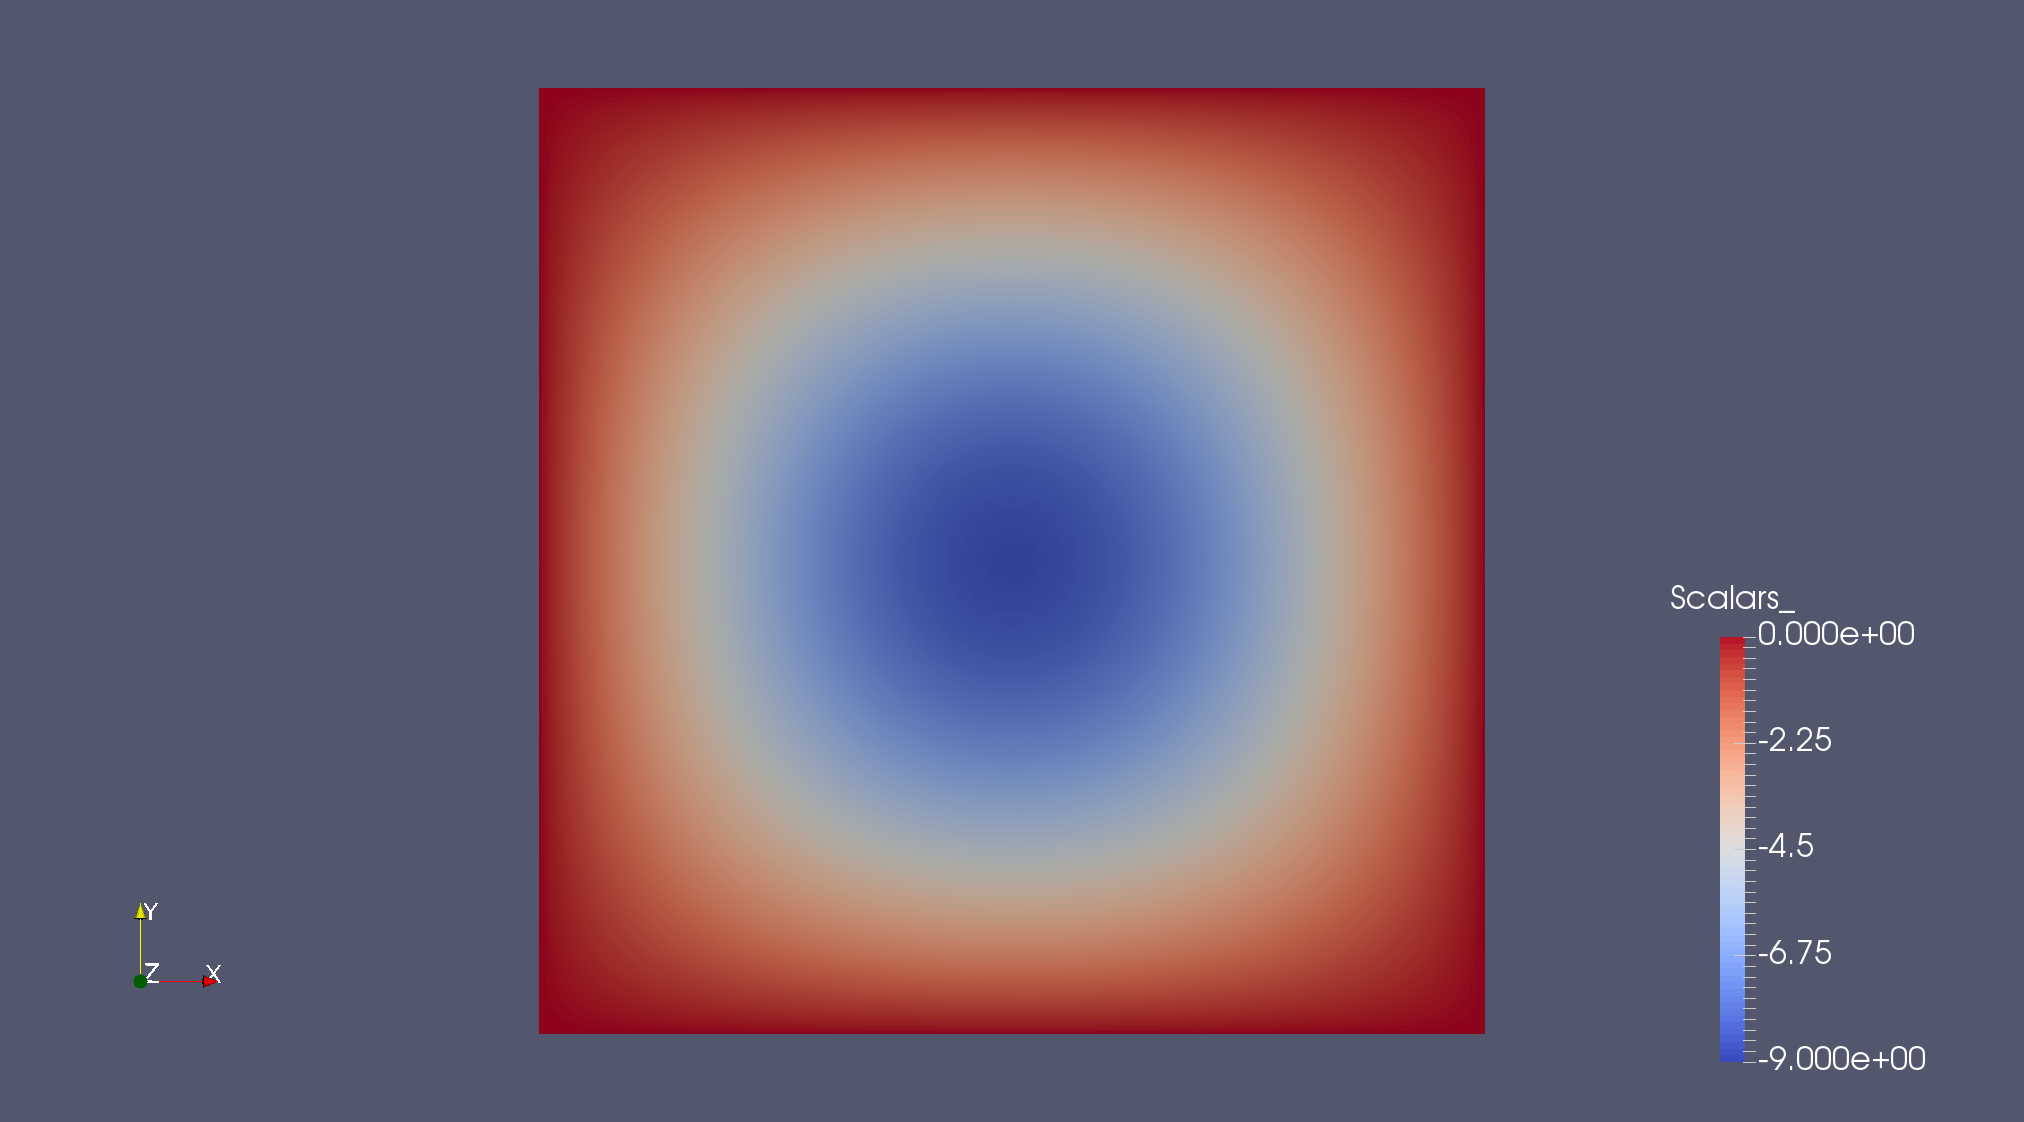
\includegraphics[width=\textwidth]{Images/symm-3r-y-0t.png}
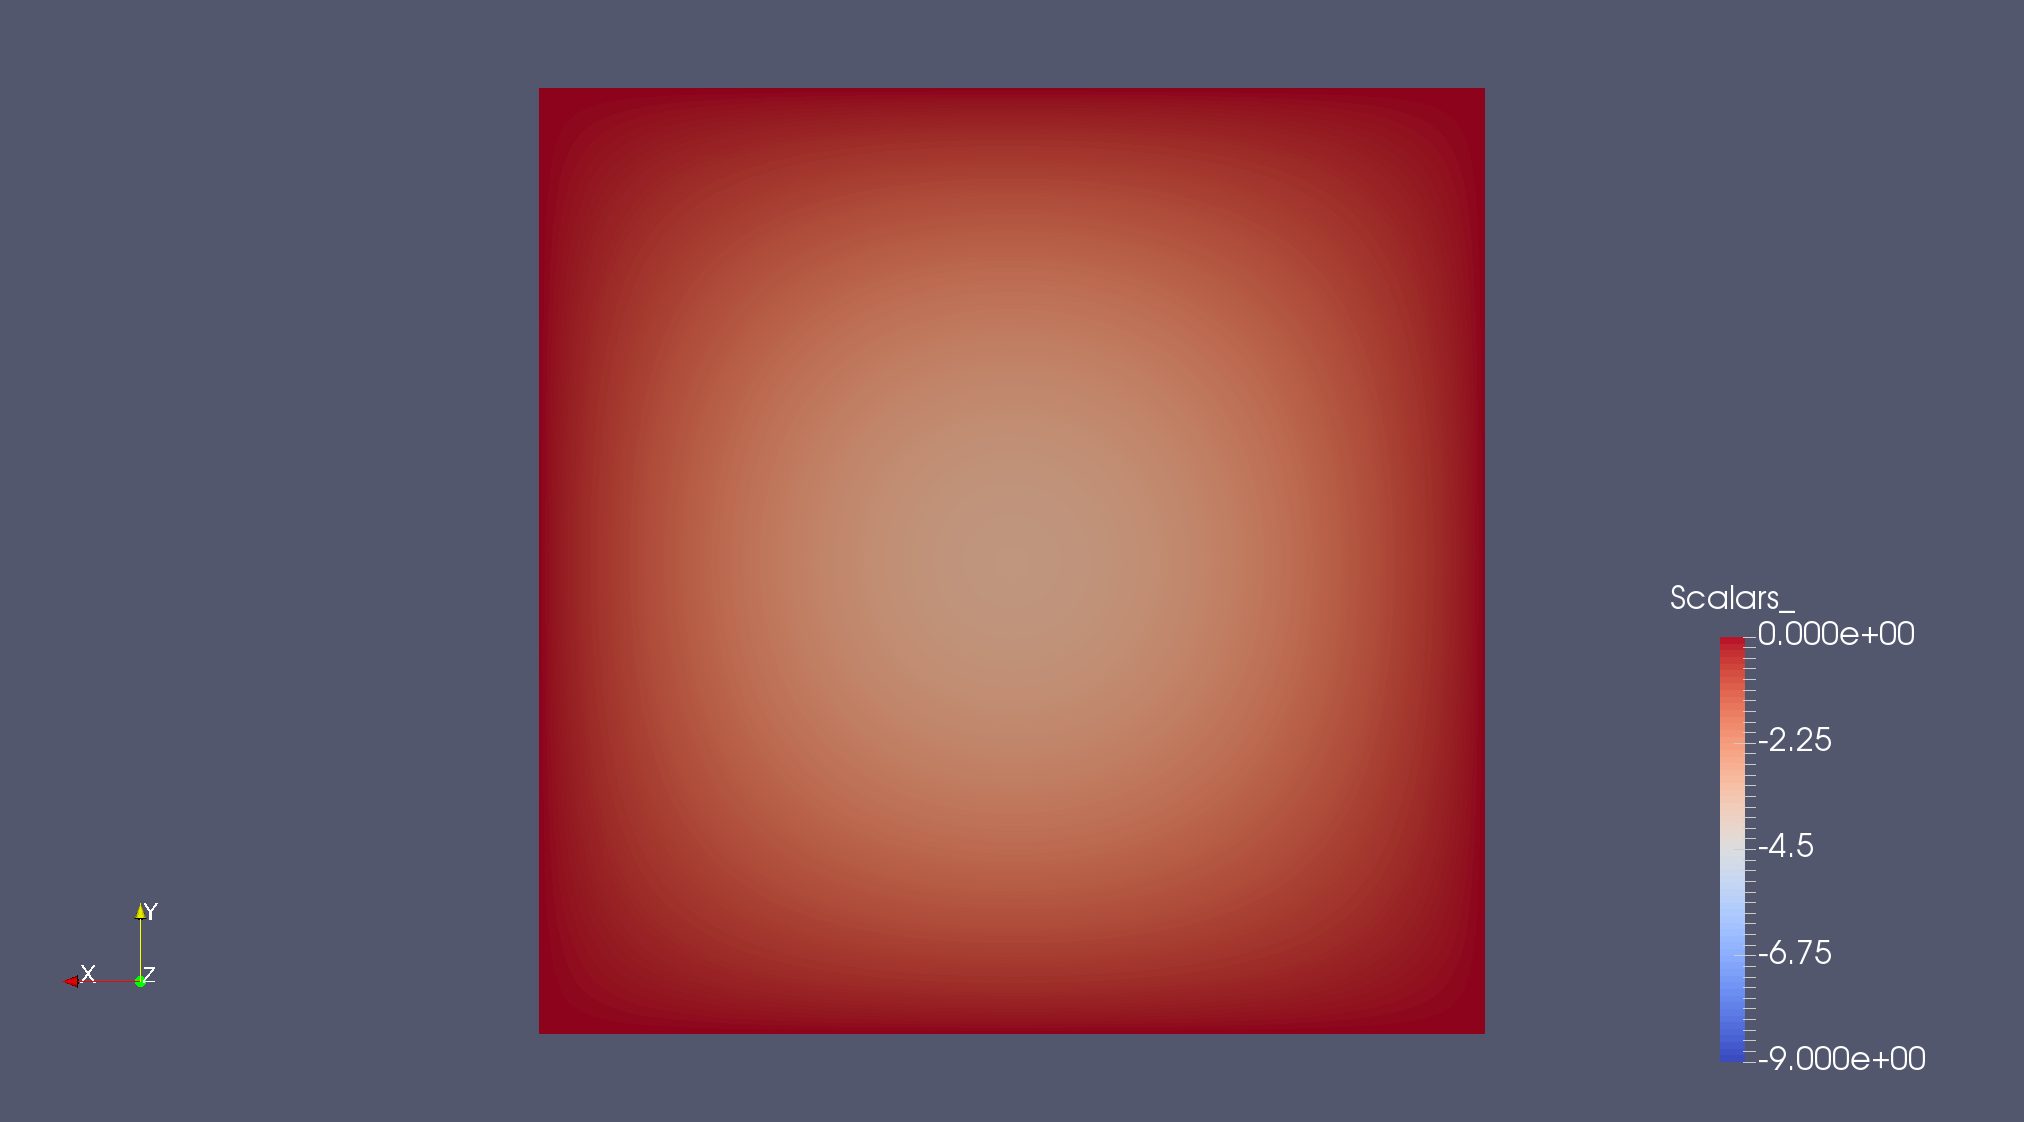
\includegraphics[width=\textwidth]{Images/symm-3r-y-Tt.png}
\caption{The state of the problem \cref{eq:symmetric-num-eq} after 3 times uniform discretization with linear basis functions, at $t = 0$ and $t = T$, respectively.}
\label{fig:symm-3r-y}
\end{figure}
\begin{figure}[htpb]
\centering
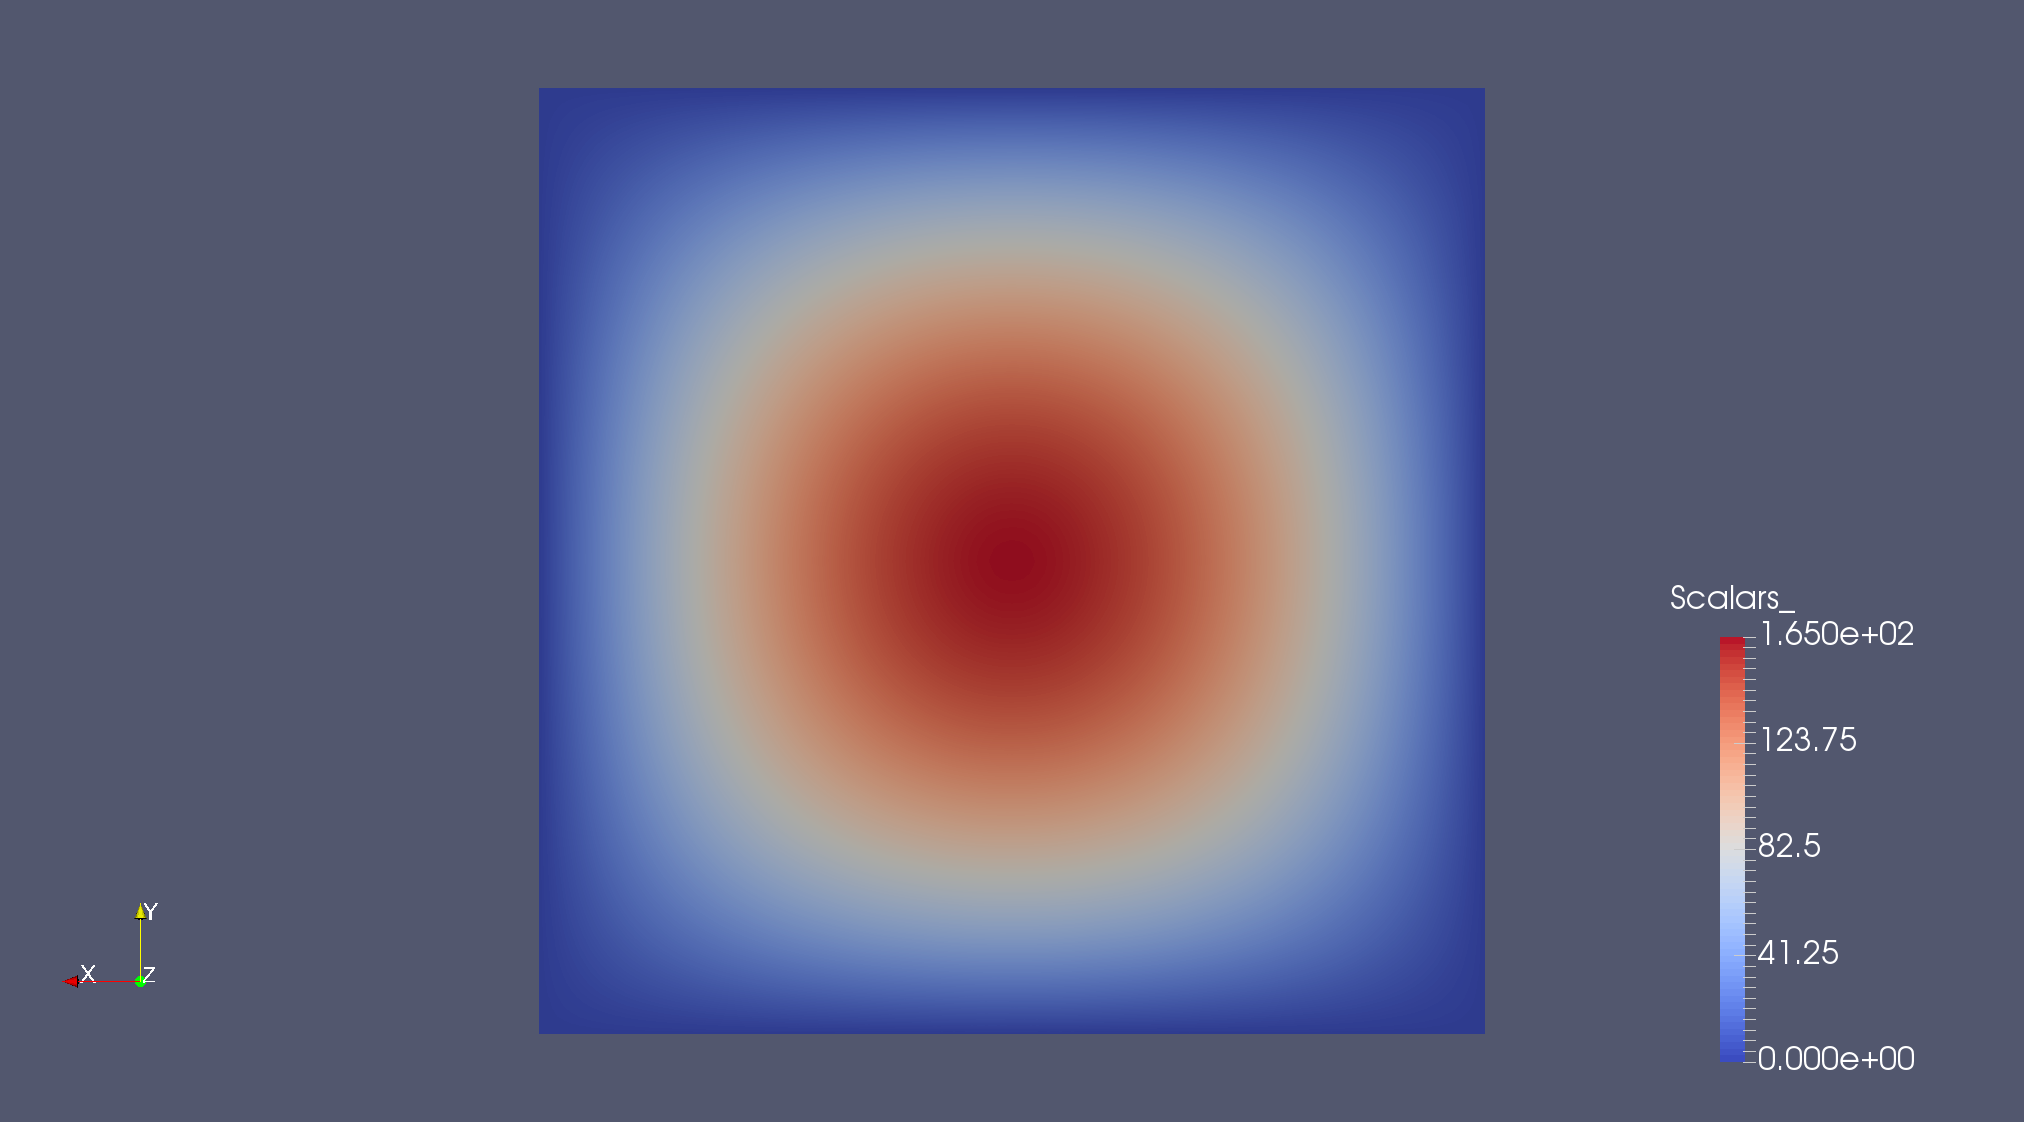
\includegraphics[width=\textwidth]{Images/symm-3r-u-0t.png}
\caption{The control of the problem \cref{eq:symmetric-num-eq} after 3 times uniform discretization with linear basis functions, at $t = 0$. At $t = T$, the control is zero by definition of the optimality system and therefore not shown here.}
\label{fig:symm-3r-u}
\end{figure}
The results in \cref{fig:symm-3r-y,fig:symm-3r-u} were solved using PARDISO by making use of the symmetric matrix formulation we gave in \cref{sec:num-unconstrained}.
\FloatBarrier
Next, we will turn towards the boundary optimal control problem discussed in \cref{sec:boundary-control-opt} and compare results in the unconstrained case and in the case that box restrictions for the control are being made.
Let $\Omega = [0, 1]^2$ and $T = 1$. Moreover, we fix the choices of $\alpha = 1$, $\lambda = 0.1$ and $\beta = 1$.
We will work with quadratic bases now.
Our problem setup shall now be $y_0 \equiv 1$ and $y_\Omega \equiv 40$.
As one would expect, all four sides of the space-time cylinder $Q$ that $u$ works on have the same solution under this setup.
\begin{figure}[htpb]
\centering
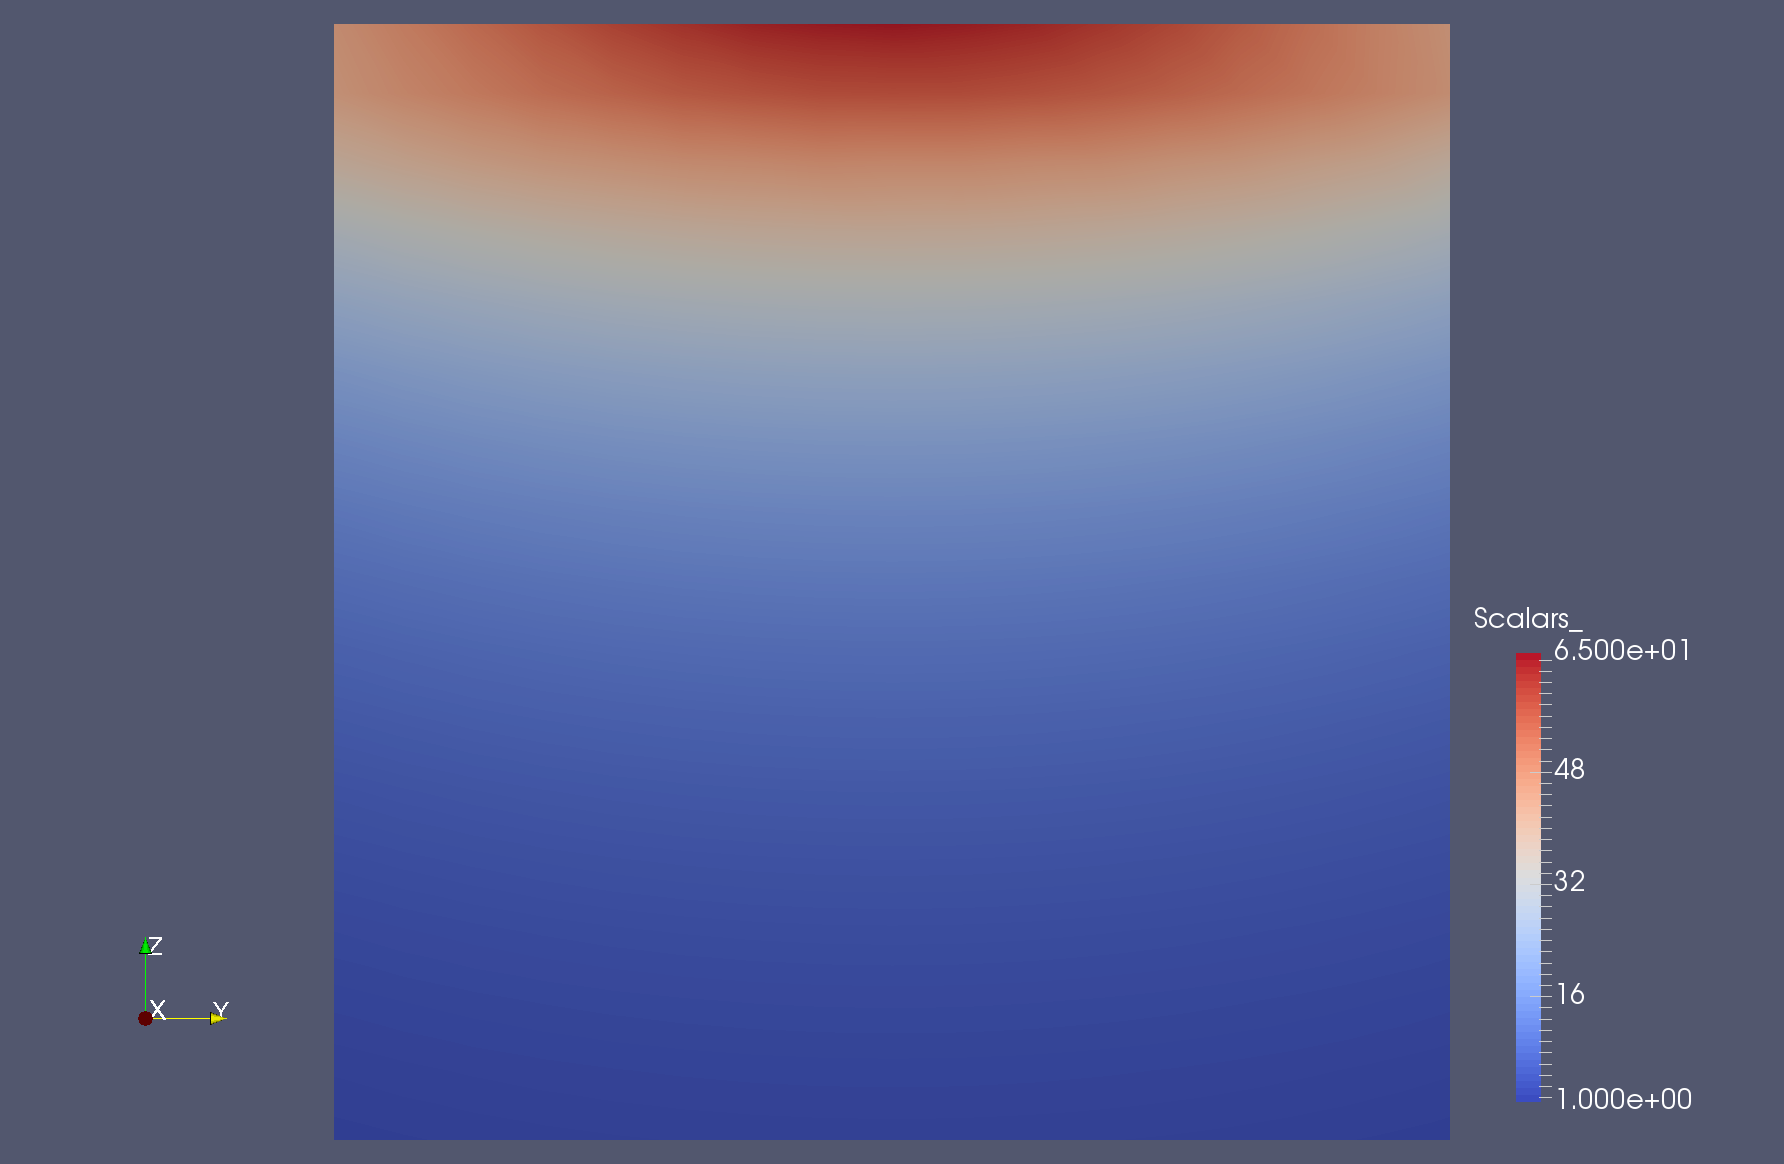
\includegraphics[width=\textwidth]{Images/boundary-const-u.png}
\caption{The control of the boundary control problem with $y_0 \equiv 1$ and $y_\Omega \equiv 40$, plotted at $\{ 1 \} \times [0, 1] \times [0, T]$.}
\label{fig:boundary-const-u}
\end{figure}
As one might expect from the fact that the control in \cref{fig:boundary-const-u} unfolds most of its energy very late on, the state changes very little until shortly before $t = T$. The reason for this is that we effectively made the thermal diffusivity mentioned in \cref{sec:OptimalControlProblem} very large corresponding to a material with physically unreasonable thermal conductivity properties.
This also means that the difference in heat from the boundary towards the center of $\Omega$ is comparatively small.
The \cref{fig:boundary-const-y-endtime} shows the state at the time point $t = T$.

Note that the optimal state does not converge towards $y_\Omega$, as we're penalizing energy required and the boundary control cannot lead towards a constant inner temperature. In fact, the center of the domain, is at the end attaining a value of roughly $30$, whereas the boundary attains values between $36$ and $37$.
In \cref{fig:boundary-const-y-cut} the state of the line $\{ 0.5 \} \times [0, 1]$ is being shown over time.
\begin{figure}[htpb]
\centering
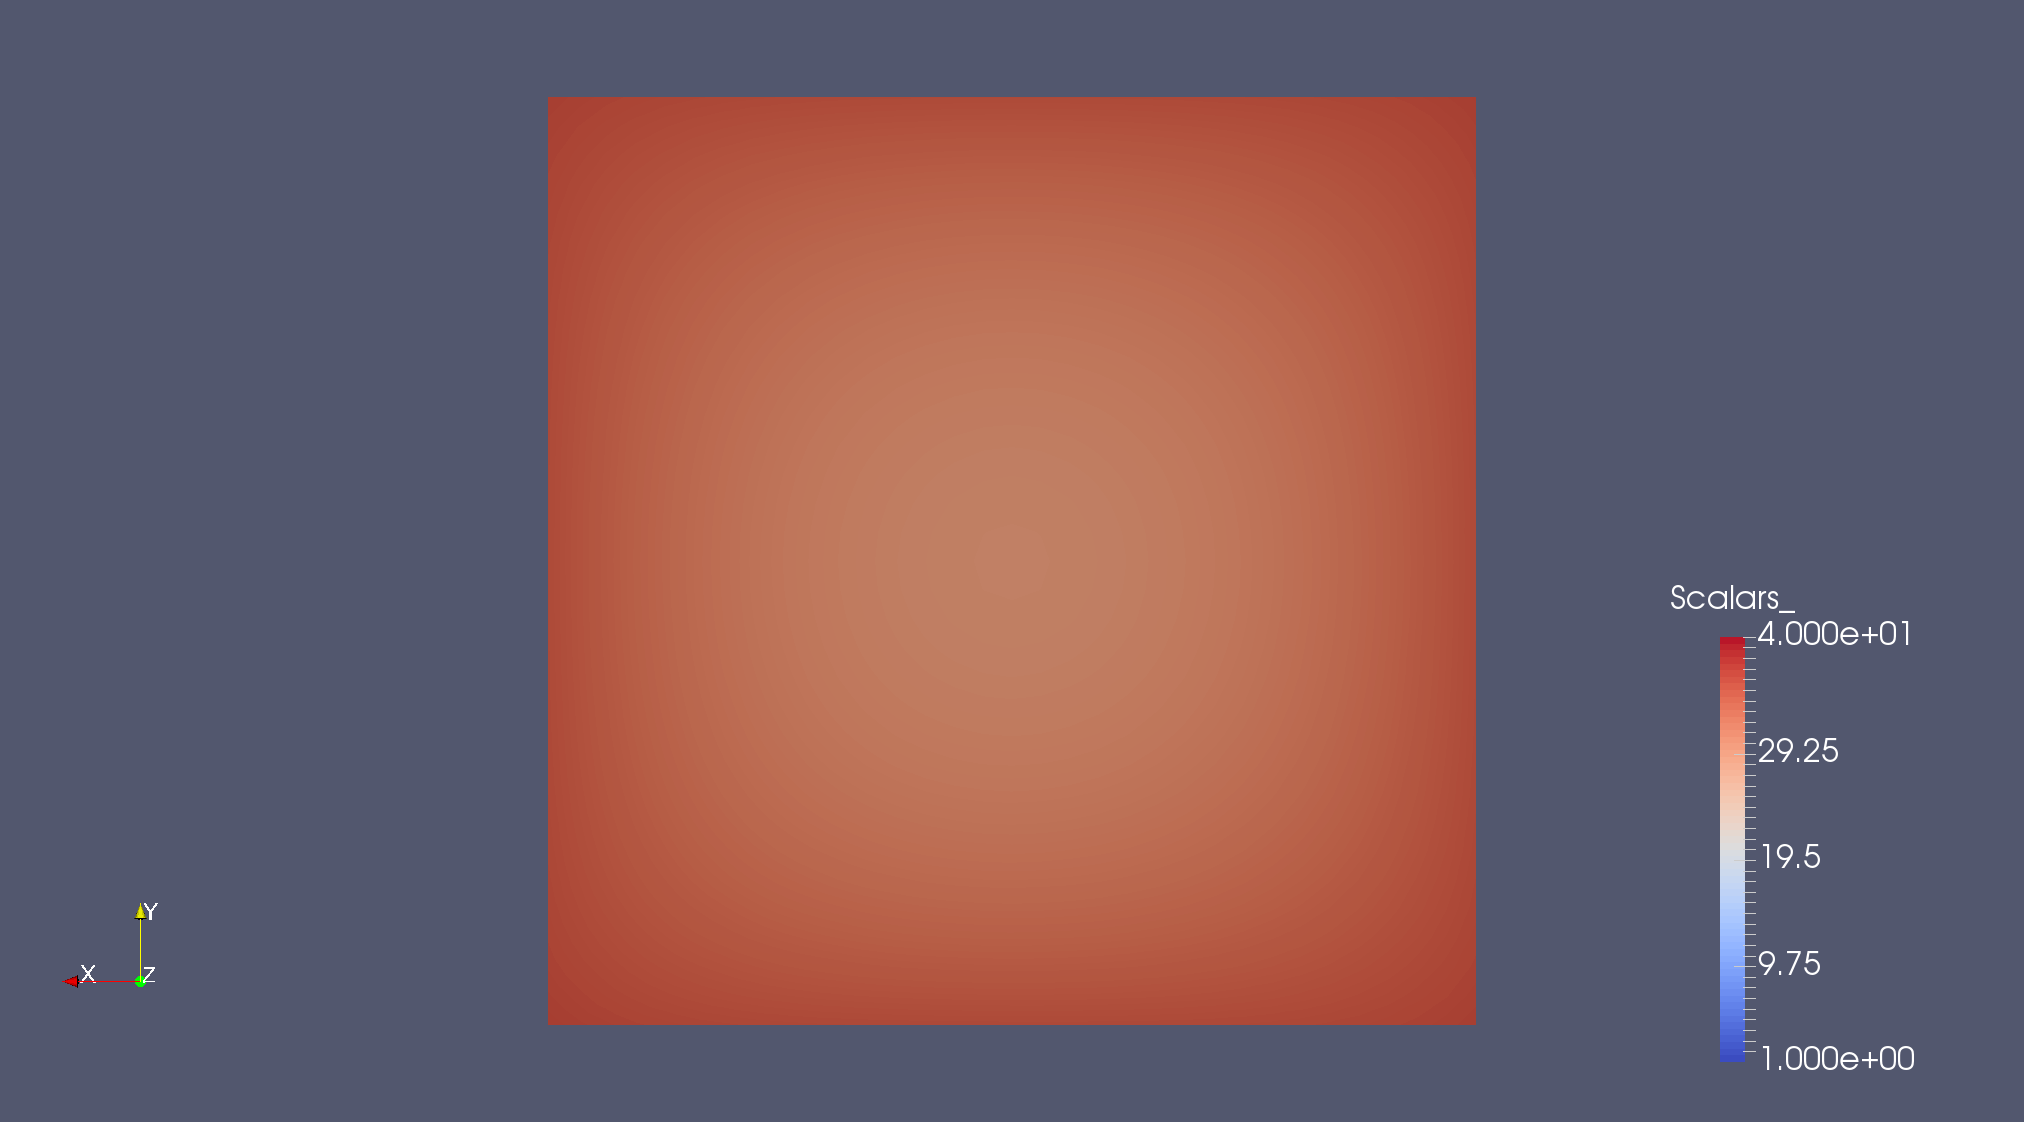
\includegraphics[width=\textwidth]{Images/boundary-const-y-endtime.png}
\caption{The state of the boundary control problem with $y_0 \equiv 1$ and $y_\Omega \equiv 40$, plotted at $t = T$.}
\label{fig:boundary-const-y-endtime}
\end{figure}
\begin{figure}[htpb]
\centering
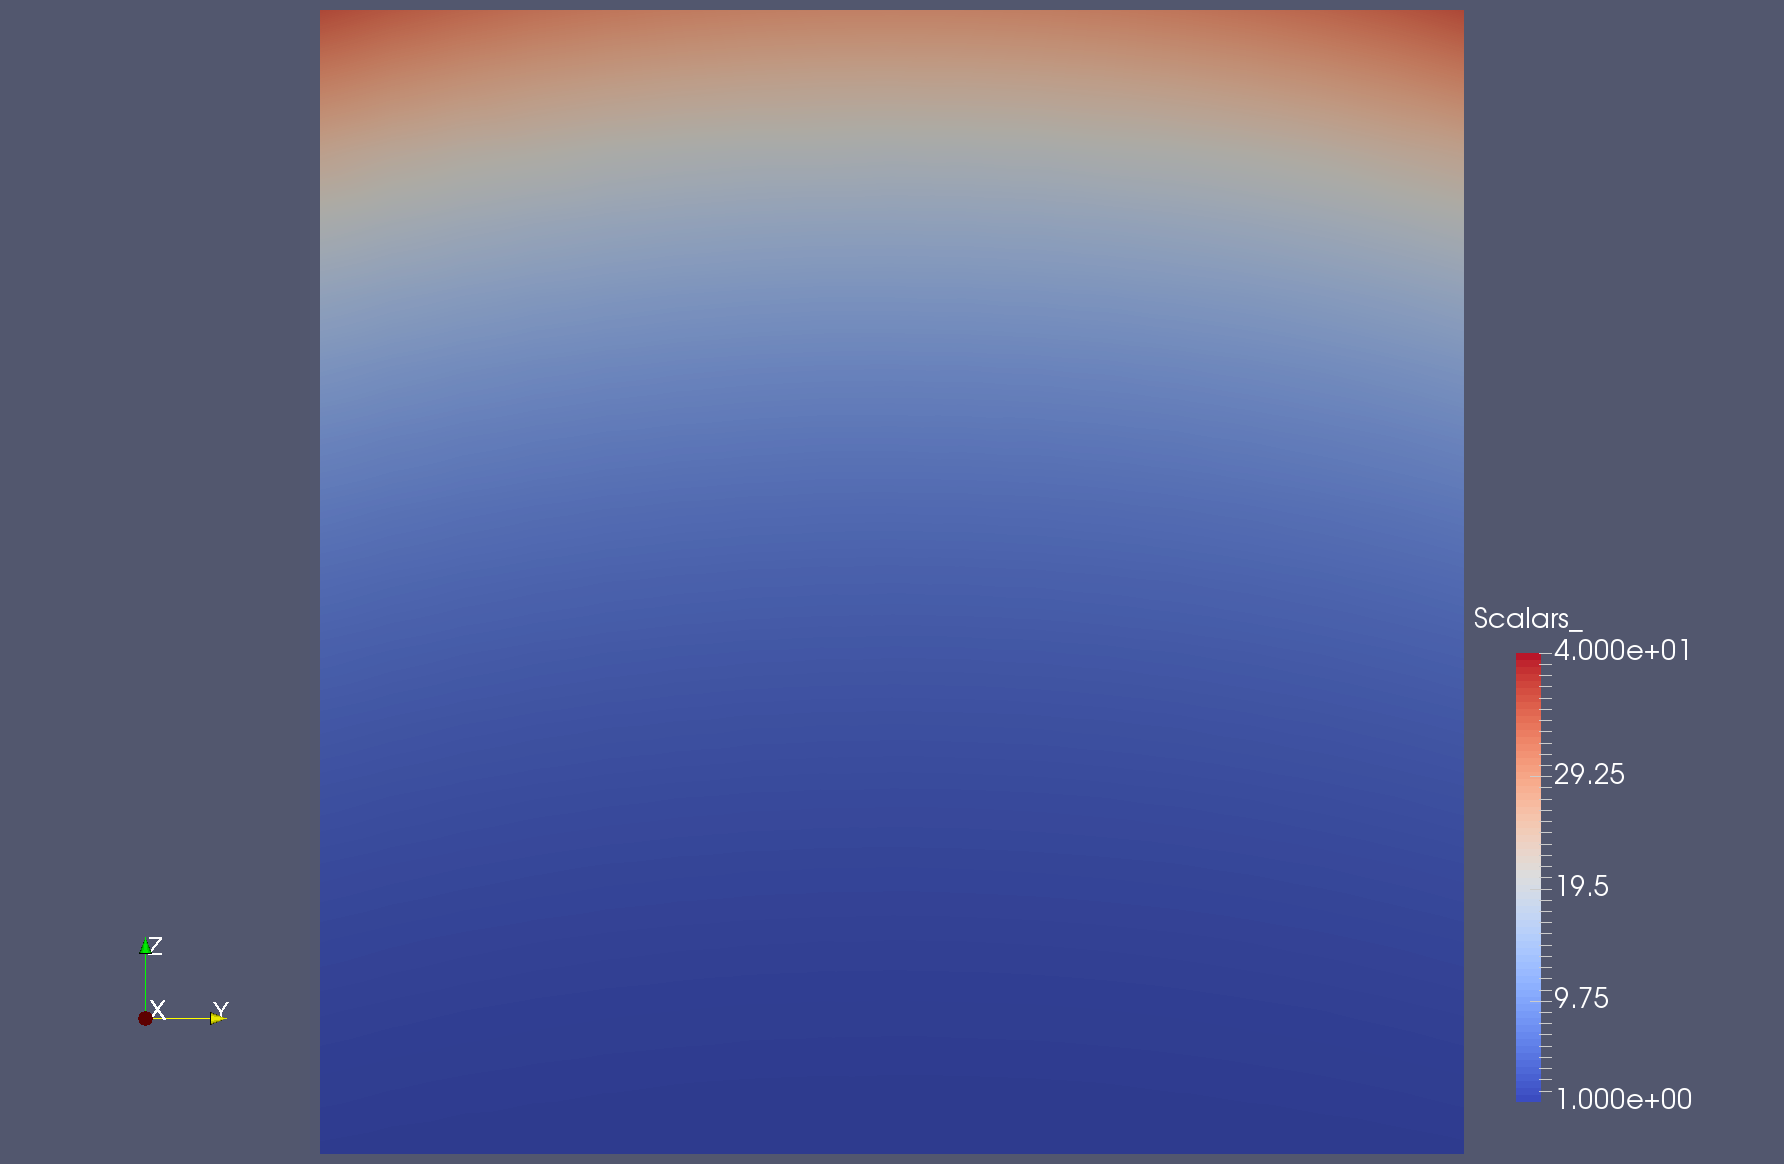
\includegraphics[width=\textwidth]{Images/boundary-const-y-cut.png}
\caption{The state of the boundary control problem with $y_0 \equiv 1$ and $y_\Omega \equiv 40$, plotted as slice $\{ 0.5 \} \times [0, 1] \times [0, 1]$.}
\label{fig:boundary-const-y-cut}
\end{figure}
\FloatBarrier

We can now use the primal-dual active set method described in \cref{sec:KR-numerics} to consider the same problem with the box restrictions $0 \leq u(x, t) \leq 40$. As we've seen, the unrestricted optimal control exceeds that value in some points, so the restricted solution should have some cut offs.
The \cref{fig:boundary-const-u-rest} shows the optimal restricted control and \cref{fig:boundary-const-y-rest-endtime} shows its associated state at $t = T$.
As given by the optimality conditions, one observes that the restricted control is the unrestricted optimal control with a cutoff taking place in the points that exceed $u_b = 40$.
Furthermore, the optimal discrete state is closer to $y_\Omega$ than the optimal unrestricted state. This is simply a result of the energy penalty. If one lowered $\lambda$ further, one would observe the difference between $\bar{y}_h(T)$ and $y_\Omega$ being much smaller.
However, in the restricted setting, the minimizer can simply require more energy as is the case here, leading to the state being closer to the desired state.
\begin{figure}[htpb]
\centering
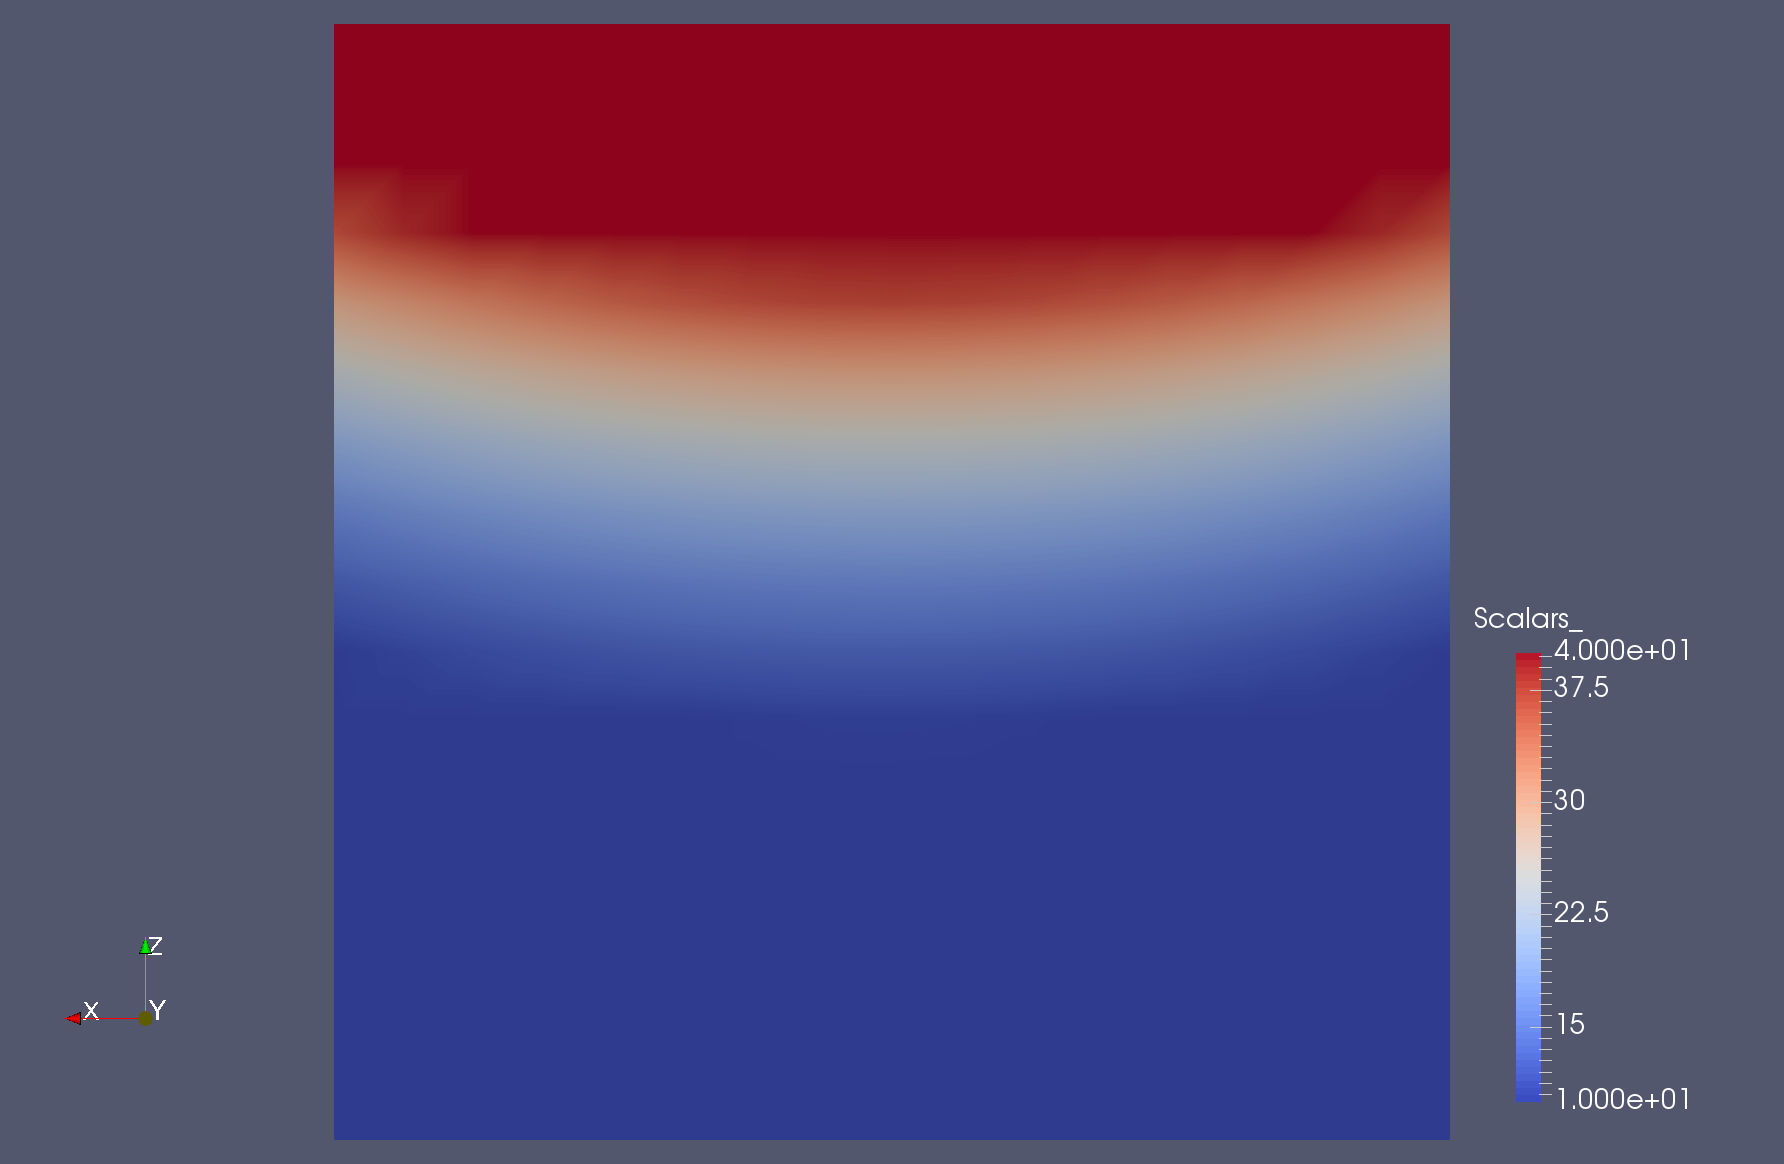
\includegraphics[width=\textwidth]{Images/boundary-cont-u-rest.png}
\caption{The control of the boundary control problem with $y_0 \equiv 1$ and $y_\Omega \equiv 40$ restricted by $0 \leq u(x, t) \leq 40$, plotted at the boundary on $[0, 1] \times \{ 1 \} \times [0, 1]$.}
\label{fig:boundary-const-u-rest}
\end{figure}
\begin{figure}[htpb]
\centering
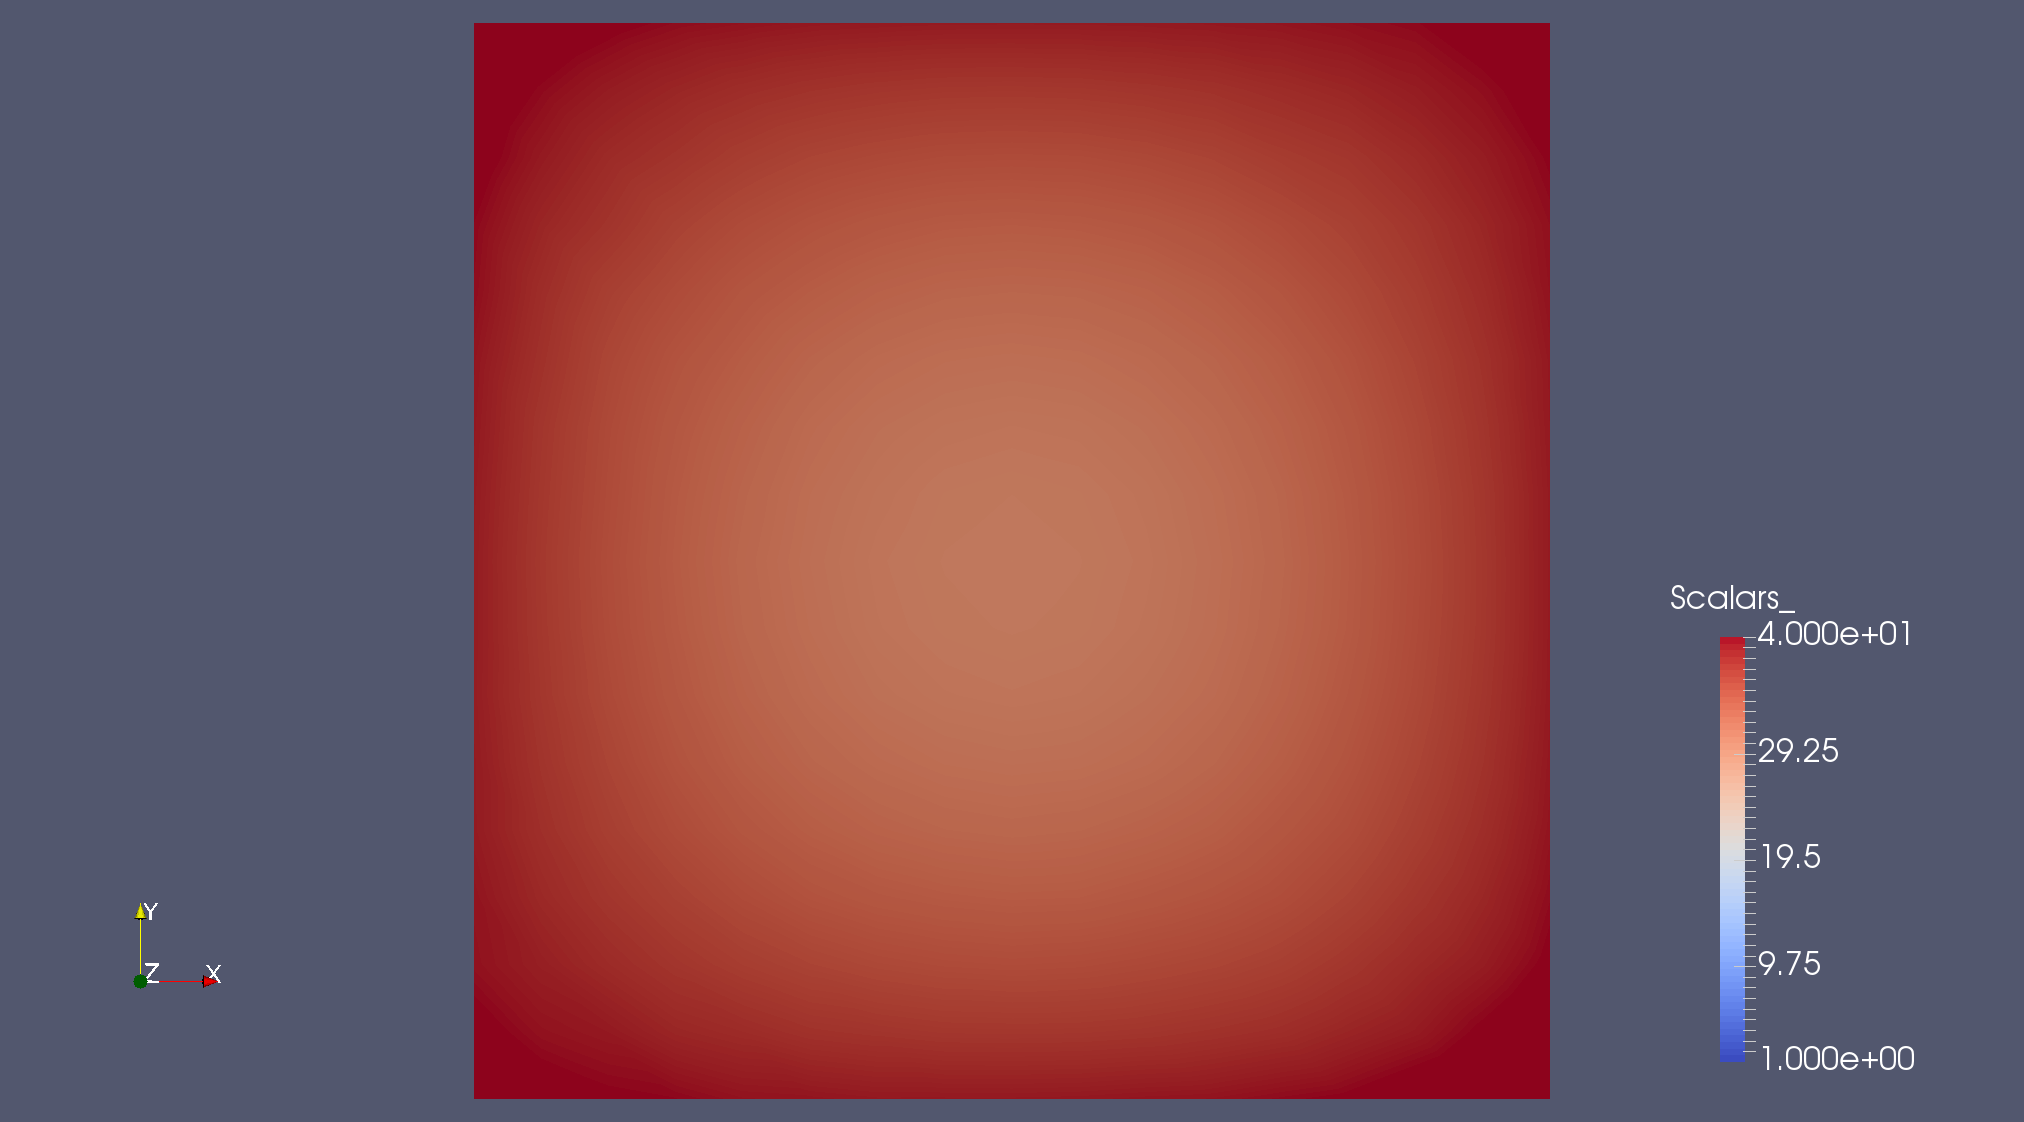
\includegraphics[width=\textwidth]{Images/boundary-cont-y-rest.png}
\caption{The state of the boundary control problem with $y_0 \equiv 1$ and $y_\Omega \equiv 40$ restricted by $0 \leq u(x, t) \leq 40$, plotted at $t = T$.}
\label{fig:boundary-const-y-rest-endtime}
\end{figure}
\end{document}